\chapter{Eye-tracking technology}
\begin{chapterabstract}
This chapter offers an~overview of how the~eye tracking process works and the~methods used along with it.
\end{chapterabstract}
%\bigskip{}

The~whole process can be divided into two parts: \emph{eye detection} and \emph{gaze estimation}. The~first step interprets the~captured images to~detect the~existence of an~eye and to~accurately find its position relative to the~head. The~next part, \emph{gaze estimation} -- uses the~calculated eye positions to~estimate \emph{gaze direction}; orientation in~space, also called \emph{Point of Regard} (PoR). \cite{hansen2010}

\medskip{}
Both parts are explained in~more detail in Sections \ref{sec:eye-detection} and \ref{sec:gaze-estimation}, respectively. 

\section{Existing techniques}
Duchowski recognises four categories of eye movement measurement methodologies: \emph{electro-oculography}, scleral contact lenses, \emph{photo/video-oculography} %or \emph{video-oculography}
and video-based combined pupil and corneal reflexion. In~his book, he briefly summarises and describes all of~them. However, the~last two categories will be covered together, because both represent video-based methods.~\cite{duchowski2007}

All current VR devices with ET use PoR measurements. %(Section \ref{sec:gaze-estimation}).
Techniques that are generally used most for that purpouse are video-based methods. This thesis will primarily focus on~describing them, but briefly mentions the~other ones first. 


\subsection{Electro-oculography}
This was the~most widely applied method to~measure eye movements in the~1970s and is still used today in~clinical settings. It~is based on~recording electric potential differences of multiple electrodes placed on the~skin around an~eye, see Figure~\ref{fig:eog} for an~example. It~offers good precision with high sampling rates \cite{cognolato2018}.

Eye movements are measured relatively to the~head, but \emph{gaze estimation} is possible if the~head is fixed at~one point in~space or if a~head position tracker is used in~parallel. The~devices used in \emph{electro-oculography} belong to a~family of intrusive devices; physical contact with the~user is required \cite{cognolato2018}. Its intrusive nature allows eye movements to~be recorded even if the~eyes are closed.

\pagebreak
\subsection{Scleral contact lens}
Techniques based on scleral contact lenses are the~most intrusive of all, but fundamentally, this makes them among the~most precise\footnote{The~accuracy is measured within arc-second units} in~terms of eye movement measurement.

The~method uses special contact lens with a~reference object attached to~it. This entire gadget is worn directly on the~eye. During the~nineteenth century, the~first attempts used lens alternatives. One~of~such was a~plaster ring, which was attached directly to~the~cornea. The~contact lens must be larger to~cover both the~cornea and the~sclera to~prevent slippage, due to~the~increase in~weight added by the~extra object. Among the~mechanical and optical attachments used, the~most popular were reflecting phosphors, line diagrams, and wire coils in magneto-optical configurations. In~particular, a~wire coil is used in the~principal method to~measure eye movements using an~electromagnetic field. An~example of a~scleral lens with wire coil can be seen in Figure~\ref{fig:contact-lens}.

The~biggest downside of a~scleral contact lens is the~discomfort of wearing one. These methods also provide eye positions relative to the~head.

\begin{figure}[!ht]\centering
    \begin{subfigure}[b]{0.45\textwidth}
        \centering
        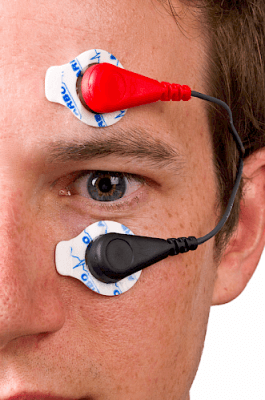
\includegraphics[width=0.51\textwidth]{img/eog.png}
        \caption{An~electro-oculography device.~\cite{fig:eog} }
        \label{fig:eog}
    \end{subfigure}
    \hfill
    \begin{subfigure}[b]{0.45\textwidth}
        \centering
        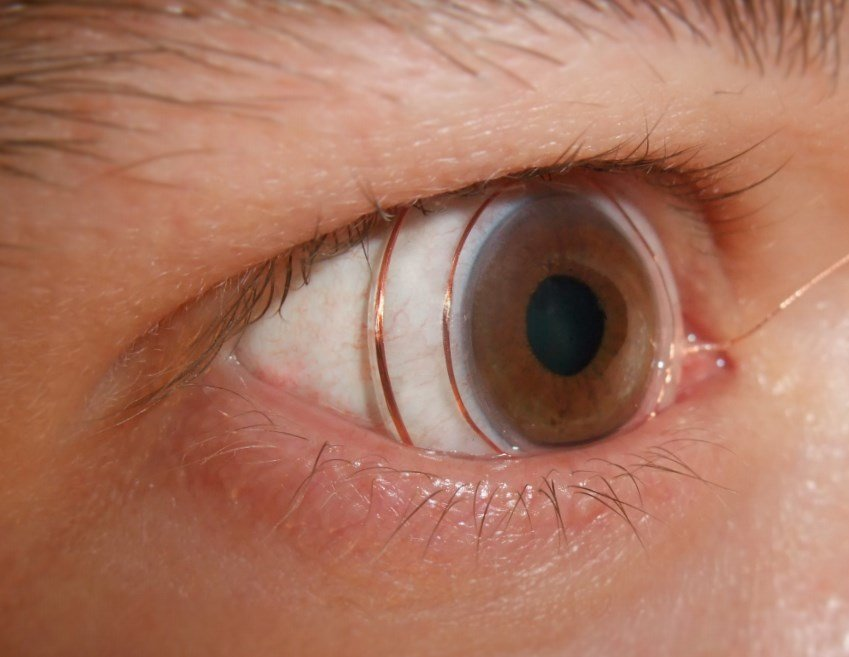
\includegraphics[width=\textwidth]{img/scleral-contact-lens.png}
        \caption{A~scleral contact lens with wire coil.~\cite{fig:scleral-lens}}
        \label{fig:contact-lens}
    \end{subfigure}
    \caption{Examples of intrusive eye tracking devices.}
\end{figure}

\begin{figure}[!ht]\centering
    \includesvg[width=0.60\textwidth]{img/basic-vod}
    \caption[Typical video-oculography setup using  method of corneal reflection.]{Typical video-oculography setup using method of corneal reflection.~\cite[p.~16497]{anuradha2017review}.}
    \label{fig:basic-vod}
\end{figure}

\subsection{Video-based methods}
\emph{Photo} and \emph{video-oculography} group together methods that record eye images with the~use of cameras or video cameras to measure eye movements. The~recording device is either attached to the~users head; head-mounted; or placed near the~user; table-mounted. Devices that are used in the~these methods are non-intrusive, even if the~device is mounted on the~head, because the~actual measurement is not made by direct physical contact with the~user.

Hansen has described video-based methods and their general process in great detail. The~publication is, despite its age, still relevant today because the~methods presented have not changed.~\cite{hansen2010}

The~idea behind video-based eye movement measurements is to~inspect distinguishable eye features from captured eye images, which must differ enough to~clearly distinguish between eye and head movements. These are the~appearance and shape of the~pupil, iris, and cornea.

%The~principles used by these features are further described in Sections \ref{sec:eye-detection} and \ref{sec:gaze-estimation}.
The~techniques that use these features are implemented using computer vision. It is possible to process them manually frame-by-frame. Doing so becomes more time-consuming, inefficient, and unreliable with each added frame. Multiple errors can be made during the~process.

The~most widely applied method for measuring eye movements is the~one based on corneal reflexion, example shown in Figure \ref{fig:basic-vod}, which involves the~use of -- at least -- one camera and a~near infrared (NIR) light source to~produce glints on the~eye cornea. The~relative position of the~glint and the~pupil centre is measured to estimate \emph{gaze direction}. Infrared (IR) light is used because it is invisible to the~naked eye and cameras can capture it. This property is useful for controlling the~lightning conditions in the~environment. It is more suited for indoor setups, where natural light can be controlled and IR rays can bounce around.
The~natural light can be also utilised for the~same purpose, but it offers a~poorer contrast~\cite{hansen2010}.

It is impossible to make an~absolutely precise gaze estimate; always a~certain deviation from the~real line of sight must be taken into account, as shown in Figure \ref{fig:basic-vod}. P represents the~pupil on the~human eye ball and G is the~glint created by the~light source. The~camera image plane is the~captured eye image, in which P and G indicate the~position of the~pupil and the~glint.~\cite{anuradha2017review}

\subsubsection*{ET process}
Each \emph{video-oculography} system must go through the~same process, shown in Figure \ref{fig:ET-process}, to~estimate \emph{gaze direction}. In the~initial step, this procedure requires image data. At least one camera is needed. The~image is processed to~determine the~existence of the~eye and to~detect its position, which can be used directly by an~application or further used to~estimate \emph{gaze direction} -- PoR, which is the~final output an~application can receive from the~system. For this to happen, the~position and rotation of the~head needs to~be tracked.

\begin{figure}[!ht]\centering{}
    \includesvg[width=0.8\textwidth]{img/ET-technique}
    \caption[Components of eye tracking process.]{Components of eye tracking process.~\cite{fig:vbprocesscomponents}}
    \label{fig:ET-process}
\end{figure}

\subsubsection*{Tracking head position}
One possible solution is to~simply sacrifice a~degree of freedom and fix the~head in one place in~space -- resting a~chin on a~raised support. It~is functional but not optimal, because there are techniques that solve this. Another device or system dedicated to~tracking the~head position needs to~be used in parallel.
If the~system is table-mounted, the~head position is already handled by some \emph{gaze estimation} algorithms. %; more about this in Section~\ref{sec:gaze-estimation}.
Meanwhile, this is impossible for head-mounted systems, because they move simultaneously with the~head, so the~\emph{gaze direction} behaves the~same. Another device or system dedicated to~tracking the~head position needs to~be used in parallel.

There are several positional tracking systems. Some track the~absolute position of the~user in a~room, such as~VICON tracker, Lighthouse from Valve, ART trackers, OptiTrack, \ldots

Other systems can detect the~position of the~head while being head-mounted. This is a~simultaneous localisation and mapping (SLAM) problem, which is solved, for example, by the Intel T265 tracking camera. However, this is beyond the~scope of this thesis.

Table-mounted devices estimate PoR on a~surface of interest -- usually a~monitor or a~TV screen -- which might be too restrictive because they cannot move with the~user and may experience difficulties registering eye positions from angles invisible to the~camera. Wearable eye gaze tracking devices use virtual scene cameras to~measure gaze in 3D space.~\cite{cognolato2018}

\section{Eye detection}
\label{sec:eye-detection}

This section derives information mainly from Hansen~\cite{hansen2010}. The~purpose of \emph{eye detection} is to~determine the~existence of the~eye and its position from the~captured eye images. It is crucial, in order to successfully perform it, to find an~eye model that is flexible enough to account for changes in the~eye's appearance without being computationally too expensive. Techniques use computer vision algorithms to analyse captured eye images to obtain information that describe the~eye's status, appearance, lighting conditions, and reflectivity. Specifically, the~viewing angle, head position, occlusion by the~eyelid, degree of eye openness, and position and colour of the~iris. These are very specific features that drastically change the~appearance of the~eye.
Eye models are determined by approaches that use the~shape or appearance of the~eye. 
%There are also hybrid ones that use both approaches and benefit from their respective advantages. 

\subsection{Shape}

These approaches create eye models using shapes of eye features. Their important characteristic is the~ability to handle changes in the~shape, scale, and rotation of the~eye. Models are defined by a~geometric shape that is either rigid or deformable, based on its parameters. 

\subsubsection*{Rigid shape}
\emph{Simple elliptical shape} is an~computationally efficient rigid model that takes advantage of the~eye features that look elliptical; iris and pupil. The~current state of those features under different viewing angles is found by edge detection algorithms. The~iris is detected by finding the~limbus, which is the~boundary between the~iris and the~sclera, and the~pupil by detecting its edge with the~iris. The~variability of these features is restricted to two degrees of freedom that describe eye movements; pan and~tilt. Higher-contrast images are preferred for easier and more precise edge detection.

\subsubsection*{Complex shape}
More detailed eye models can be made for greater precision. Methods based on a~deformable eye model use for the~eye description generic deformable template, which is modifiable with parameters. One method is used to represent the~eyelids and the~iris. The~former is described by two parabolas with 11 parameters, while the~iris is a~simple circle. Another method describes the~deformable eye with two semiellipses that are defined by six parameters. 

Methods based on a~deformable eye model offer an~accurate and generic representation of the~eye, but they are computationally very demanding and require high contrast images that are taken from a~close distance to the~eye for their proper operation. Algorithms solving these issues incorporate energy minimisation processes of computer vision. The~same approaches are applicable to face recognition. 

\subsection{Appearance}

Appearance-based approaches detect and track eyes directly from captured images, as opposed to shape approaches. The~eye and its features are described by the~colour distribution in the~image or by the~results of \emph{image filters}. The~computer vision techniques employed do not require any knowledge about the~eye itself. These are actually able to model absolutely anything. The~requirement to train a~model is to use a~sufficiently large set of images that represent the~appearance of the~desired object. 
%when the~model is trained on a~sufficiently large dataset of images representing the~appearance of the~desired object.

Methods based on these approaches can have problems with rotation, scale, and detection of the~eye. The~reason for this may be the~insufficient amount and diversity of training data that do not reflect different types of eyes, head orientations, or lighting conditions. 

Information about the~appearance of the~eye is extracted from captured images either directly or by their transformation, which can enhance the~features of the~eye or suppress differences in illumination.

\pagebreak{}
\subsubsection*{Image filtering}
\emph{Image filtering} are techniques used to~modify raster images, either over the~entire image or just in a~selected area. Filtering can be done in two ways, either by filtering only one pixel value or by adjusting a~pixel, based on its near surrounding neighbours. These techniques include, for example, brightness and contrast adjustments, gamma correction, thresholding, blurring, edge detection, and convolution.~\cite{trnka2020thesis}

\subsubsection*{Eye features}
Captured eye data can be transformed by filters. Filter responses to a~given image can also be used for individual eye features. Some are more appropriate than others. Limbus boundary detection is easily implementable but offers low precision~\cite{cognolato2018}. Generally, explicit eye edge detection may not always be correctly detected due to changes in light, image focus, occlusion, or eyelid cover.

Eye images taken from a~reasonably close distance allow the~pupil to be a~reliable feature. It depends on the~pupil, and the~iris appears darker than in other areas. This might require higher-contrast images. One method uses an~iterative threshold algorithm that searches for two dark regions. However, this method alone is insufficient in some cases. It could confuse the~pupil with areas with dark shadows, eyebrows, or even areas of individuals with darker skin. There is an~improvement for this method that uses an~NIR light source.

\subsection{Dark and Bright pupil}
\label{sec:dp-method}

These are two methods that extend the~eye detection method by localisation of the~pupil with an~IR light ray. It is used to increase the~pupil contrast in captured images for more robust eye detection.

The~methods depend on the~angle of light entering the~pupil. When the~IR light bounces back from the~eye to the~camera, the~pupil brightens up. On the~contrary, when the~light is at an~angle away from the~camera, it creates an~effect where the~pupil appears much darker. 

This Czech thesis presents an~implementation of the~dark pupil method using a~\emph{convolutional neural network} (CNN)~\cite{trnka2020thesis}.

\subsection{Purkinje images}
Another characteristic of the~eye that is observed is the~behaviour of how light reflects off its surface. These features were found by Jan Evangelista Purkyně. They are named after him and called \emph{Purkinje images}. In the~context of ET, IR light is used to produce different types of reflexions on the~eye, which are then detected by algorithms.

Exactly four distinct \emph{Purkinje images} can be recognised. First one (P1) is reffered to as a~glint, which is reflexion of the~outer side of the~cornea. Second (P2) is the~reflexion from the~back side of the~cornea. Third (P3) bounces off the~front side of the~eye lens. Fourth (P4) image captures the~reflectivity of the~back side of the~eye lens.~\cite{ugwitz2020thesis}

\pagebreak{}

\section{Gaze estimation}
\label{sec:gaze-estimation}
Determining gaze is to be understood as the~gaze direction or PoR, which is a~2D coordinate on a~surface. \emph{Pupil Centre Cornea Reflexion} (PCCR) is a~method that uses an~NIR light source to produce the~first Purkinje images while simultaneously darkening the~pupil using the~dark pupil method. This results in a~very contrasting image of a~glint and a~pupil. These features are easy to detect, so their positions are determined. It is the~most widely used ET method to date~\cite{tobii-eye-trackers}. Gaze is estimated by their relative position, which is used by two different methods.~\cite{cognolato2018}

However, the~position and orientation of the~head need to be taken into account for systems that do not operate with a~fixed head. In these cases, the~head movement must be compensated for. This problem is not solved with HMD systems because they move simultaneously with the~head.~\cite{anuradha2017review}

\subsection{2D regression}

2D regression is a~group of methods that use the~position of the~pupil and the~glint of the~eye to map directly to a~PoR. This mapping is expressed by some polynomial function or by a~neural network. There are 2D regression methods that are capable of head compensation during polynomial mapping~\cite{anuradha2017review}. Some are able to address this by adding an~additional camera, which requires stereo calibration~\cite{hansen2010}.

For these methods, it is essential to use a~calibration for the~polynomial function. It is often based on several points on the~screen that are spaced around. The~points cause the~eye to look in a~certain direction. The~camera records the~eye. From this eye image, the~position of the~pupil, the~glint and their relative vector are determined and assigned to a certain gaze vector or PoR on the~screen according to a~specific calibration point. This operation finds the~correct parameters for the~polynomial function from them. The~accuracy of gaze estimation is improved with a~larger number of calibration points.~\cite{anuradha2017review}

\subsection{3D model}
Then there are methods that create a~geometric 3D model of the~eye from the~detected features, and the~estimated gaze originates from the~centre of the~cornea as the~optical axis of this 3D model. These methods utilise the~similarity of the~shape and size of the~eyes.~\cite{anuradha2017review} 

For the~complete construction of the~model, knowledge of the~camera position and light is required, which can be obtained by calibration. For cases where the~head position keeps changing, the~head position must be constantly evaluated. External positioning systems can be useful for this. The~basic device that uses a~3D model to estimate gaze is one IR camera and one IR LED. Such a~solution might require calibration. However, there are many other solutions that add multiple LEDs and cameras to the~system that might no longer require a~calibration. If it does, only once in a~while. For example, if multiple users are using the~device, each would need their own calibration. As the~number of cameras and LEDs increases, so does the~accuracy and quality of the~measurement, while the~need for calibration decreases.~\cite{trnka2020thesis}
